\chapter{Theoretical introduction}
	
\section{Problem introduction}
 Theoretical introduction to a problem and mathematical concepts, literature review.... \\
 
 \noindent General task is to predict a weather state $\Omega$ at a timestamp $t$, based on \emph{s} steps into the past - previous weather states: $(\Omega_{t-1}, ..., \Omega_{t-s})$.
 As a $\Omega$ we define a multidimensional vector of a shape: (latitude span, longitude span, features). Spatial span was selected so as to cover the border of the whole of Poland and some of its neighbors. More details are discussed in dataset chapter [href].

\section{Literature review}
Short review of quality papers related to this problem; explanation of what was already achieved in this task - STATA solutions, especially emphasizing GraphCast paper; what we want to reproduce or compare ourself with.
 
 \subsection{Naming convention}
 For further convenience, we propose a general naming convention. We define a $\mathbf{\Phi}$ as a set of baseline models that consist of: 
 \begin{itemize}
    \item $\mathbf{\Phi}_{slr}$ - Simple Linear Regression,
    \item $\mathbf{\Phi}_{lr}$ - Linear Regression,
    \item $\mathbf{\Phi}_{es}$ - Exponential Smoothing,
    \item $\mathbf{\Phi}_{lgb}$ - Light Gradient Boosting Trees,
 \end{itemize}
 
 \noindent Additionally, due to the fact that model $\mathbf{\Phi}_i$ is separated into independent models that predicts single feature $f_j$ of a weather state: 
 \[
 \mathbf{\Phi}_{i} = (\mathbf{\Phi}_{i}^{f_1}, ..., \mathbf{\Phi}_{i}^{f_n})
 \]
 In further considerations, we will use a term \textbf{sub-models} for each of $\mathbf{\Phi}_{i}^{f_j}$.

 \newpage
 \section{Autoregression}
 \noindent Each baseline model is designed to predict the entire weather state for only the next timestamp - unit forecasting horizon. Therefore, when applying our models for short-term prediction task of a few timestamps into the future, the autoregressive approach is commonsensical. \\ \\
 
 \noindent Let's define model input as $\mathbf{X}$, a vector of $s$ weather states: 
 \[
 \mathbf{X} = (X_{t}, ..., X_{t+s-1})
 \]
 and output of a model as $\mathbf{\hat{Y}}$, which consist of $fh$ forecasted states:
 \[
 \mathbf{\hat{Y}} = (\hat{Y}_{t+s}, ..., \hat{Y}_{t+s+fh-1})
 \]
 
 \noindent Autoregressive prediction is $fh$-steps process such that:
 \begin{flalign*}
    &\hat{Y}_{t+s} = \mathbf{\Phi}_{i}(X_{t}, ..., X_{t+s-1}) \\
    &\hat{Y}_{t+s+1} = \mathbf{\Phi}_{i}(X_{t+1}, ..., X_{t+s-1}, \hat{Y}_{t+s}) \\
    &\vdots \\
    &\hat{Y}_{t+s+fh-1} = \mathbf{\Phi}_{i}(X_{t+fh-1}, ...,  \hat{Y}_{t+s+fh-3}, \hat{Y}_{t+s+fh-2})
 \end{flalign*}
 
 \noindent For each model except $\mathbf{\Phi}_{slr}$, during every autoregressive step concatenation of outputs from sub-models is required, whereas $X_t$ needs to have information from every feature:
 \begin{flalign*}
    &\hat{y}_t^{f_i} = \mathbf{\Phi}_{j}^{f_i}(\mathbf{X}) \\
    &\hat{Y}_{t} = (\hat{y}_t^{f_0}, ..., \hat{y}_t^{f_n}) \\
 \end{flalign*}
 
\newpage
\section{Neighbors}
Explain neighbors concept used in baselines ... \\

\noindent For each input matrix we've implemented though called neighbors feature. It is expanding each of our data points to store information about closely located grid boxes. They're chosen based on the relative distance (radius) between the center of grid-boxes: $r$. On underneath figure, grid boxes colored grey represents relative data point and black boxes are its neighbors.

\begin{figure}[h!]
    \centering

    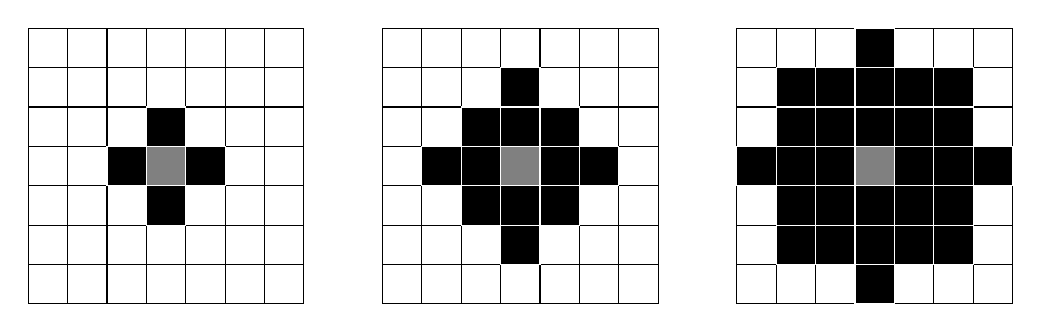
\begin{tikzpicture}[scale=0.5]
        \draw[step=1, black] (0,0) grid (7,7);
        \filldraw[fill=gray, draw=white] (3,3) rectangle (4,4);
        \filldraw[fill=black, draw=white] (3,2) rectangle (4,3);
        \filldraw[fill=black, draw=white] (2,3) rectangle (3,4);
        \filldraw[fill=black, draw=white] (3,4) rectangle (4,5);
        \filldraw[fill=black, draw=white] (4,3) rectangle (5,4);
        
        \begin{scope}[shift={(9,0)}]
            \draw[step=1, black] (0,0) grid (7,7);
            \foreach \i in {1, ..., 9} {
                \pgfmathtruncatemacro\row{mod(\i-1,3)}
                \pgfmathtruncatemacro\col{int((\i-1)/3)}
                \filldraw[fill=black, draw=white] (\row+2,\col+2) rectangle (\row+3,\col+3);
            }
            \filldraw[fill=gray, draw=white] (3,3) rectangle (4,4);
            \filldraw[fill=black, draw=white] (1,3) rectangle (2,4);
            \filldraw[fill=black, draw=white] (5,3) rectangle (6,4);
            \filldraw[fill=black, draw=white] (3,1) rectangle (4,2);
            \filldraw[fill=black, draw=white] (3,5) rectangle (4,6);
        \end{scope}

        \begin{scope}[shift={(18,0)}]
            \draw[step=1, black] (0,0) grid (7,7);
            \foreach \i in {1, ..., 25} {
                \pgfmathtruncatemacro\row{mod(\i-1,5)}
                \pgfmathtruncatemacro\col{int((\i-1)/5)}
                \filldraw[fill=black, draw=white] (\row+1,\col+1) rectangle (\row+2,\col+2);
            }
            \filldraw[fill=gray, draw=white] (3,3) rectangle (4,4); 
            \filldraw[fill=black, draw=white] (0,3) rectangle (1,4);
            \filldraw[fill=black, draw=white] (6,3) rectangle (7,4);
            \filldraw[fill=black, draw=white] (3,0) rectangle (4,1);
            \filldraw[fill=black, draw=white] (3,6) rectangle (4,7);
        \end{scope}
    \end{tikzpicture}
    \caption{Neighbors logic for $r=(1,2,3)$}
\end{figure}

\noindent Unfortunately, the trade-off between memory footprint, computational complexity, and performance gain was not sufficient to incorporate and test bigger $r$ values.
 
 \section{Baselines}
 \subsection{Exponential Smoothing}
 \subsection{Simple Linear Regression}
 \subsection{Linear Regression}
 
 \[
    \mathbf{X} \boldsymbol\beta = \mathbf{\hat{Y}}
 \]
 
 \[
    \begin{bmatrix}
    x_{11} & x_{12} & \cdots & x_{1n}\\
    x_{21} & x_{22} & \cdots & x_{2n}\\
    \vdots & \vdots & \ddots & \vdots\\
    x_{n1} & x_{n2} & \cdots & x_{nn}
    \end{bmatrix}
    \begin{bmatrix}
    \beta_1\\\beta_2\\ \vdots\\b_n
    \end{bmatrix}
    =\begin{bmatrix}
    \hat{y_1}\\\hat{y_2}\\ \vdots\\\hat{y_n}
    \end{bmatrix}
\]
 \subsection{LGBM}
 \subsection{UNet}


\section{Neural network concept}
Explain architecture of dense neural networks and other types such as convolutional, recurrent, graph (depending on which one eventually will be used).

\section{GraphCast}
Deep dive into GraphCast architecture.

\section{Model}
Proposed model architecture and comparision with GraphCast. 
	